\documentclass[b5paper, 9pt, twocolumn, titlepage]{jsbook}
\usepackage[dvipdfmx]{graphicx,color,hyperref}
\usepackage{url}
\usepackage{amssymb}
\usepackage{amsmath}
\usepackage{multirow}
\usepackage{pxjahyper}%pdfのしおりの文字化けを防止する.内部コードを判別して切り替えてくれる
\usepackage{comment}
\usepackage{listings}
\graphicspath{{figs/}}

\title{CNC切削加工入門}
\author{文責:ワッシャー (twitter:@ntm510)}

\begin{document}

\pagestyle{empty}
\maketitle
\thispagestyle{empty}
\sloppy

\section*{初めに}

本稿はプログレスレポートのテンプレートである\cite{Sakai}.
p
本稿における「,」や「.」は,\verb|make pub|を実行することで,「,」や「.」に変更される.

図は\figref{nowprinting}や\tabref{sample}として参照する.

\begin{figure}[tbh]
 \begin{center}
  \begin{minipage}{0.3\columnwidth}
   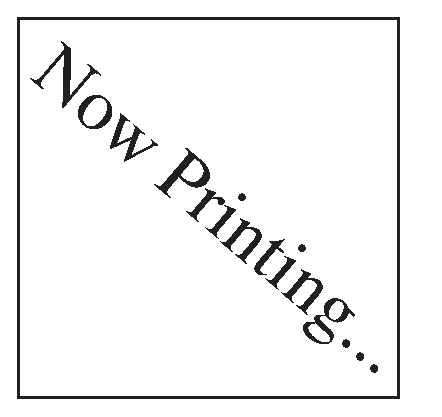
\includegraphics[width=\columnwidth]{nowprinting.eps}
   \caption{eps図の参考例}
  \end{minipage}
  \hspace{0.15\columnwidth}
  \begin{minipage}{0.3\columnwidth}
   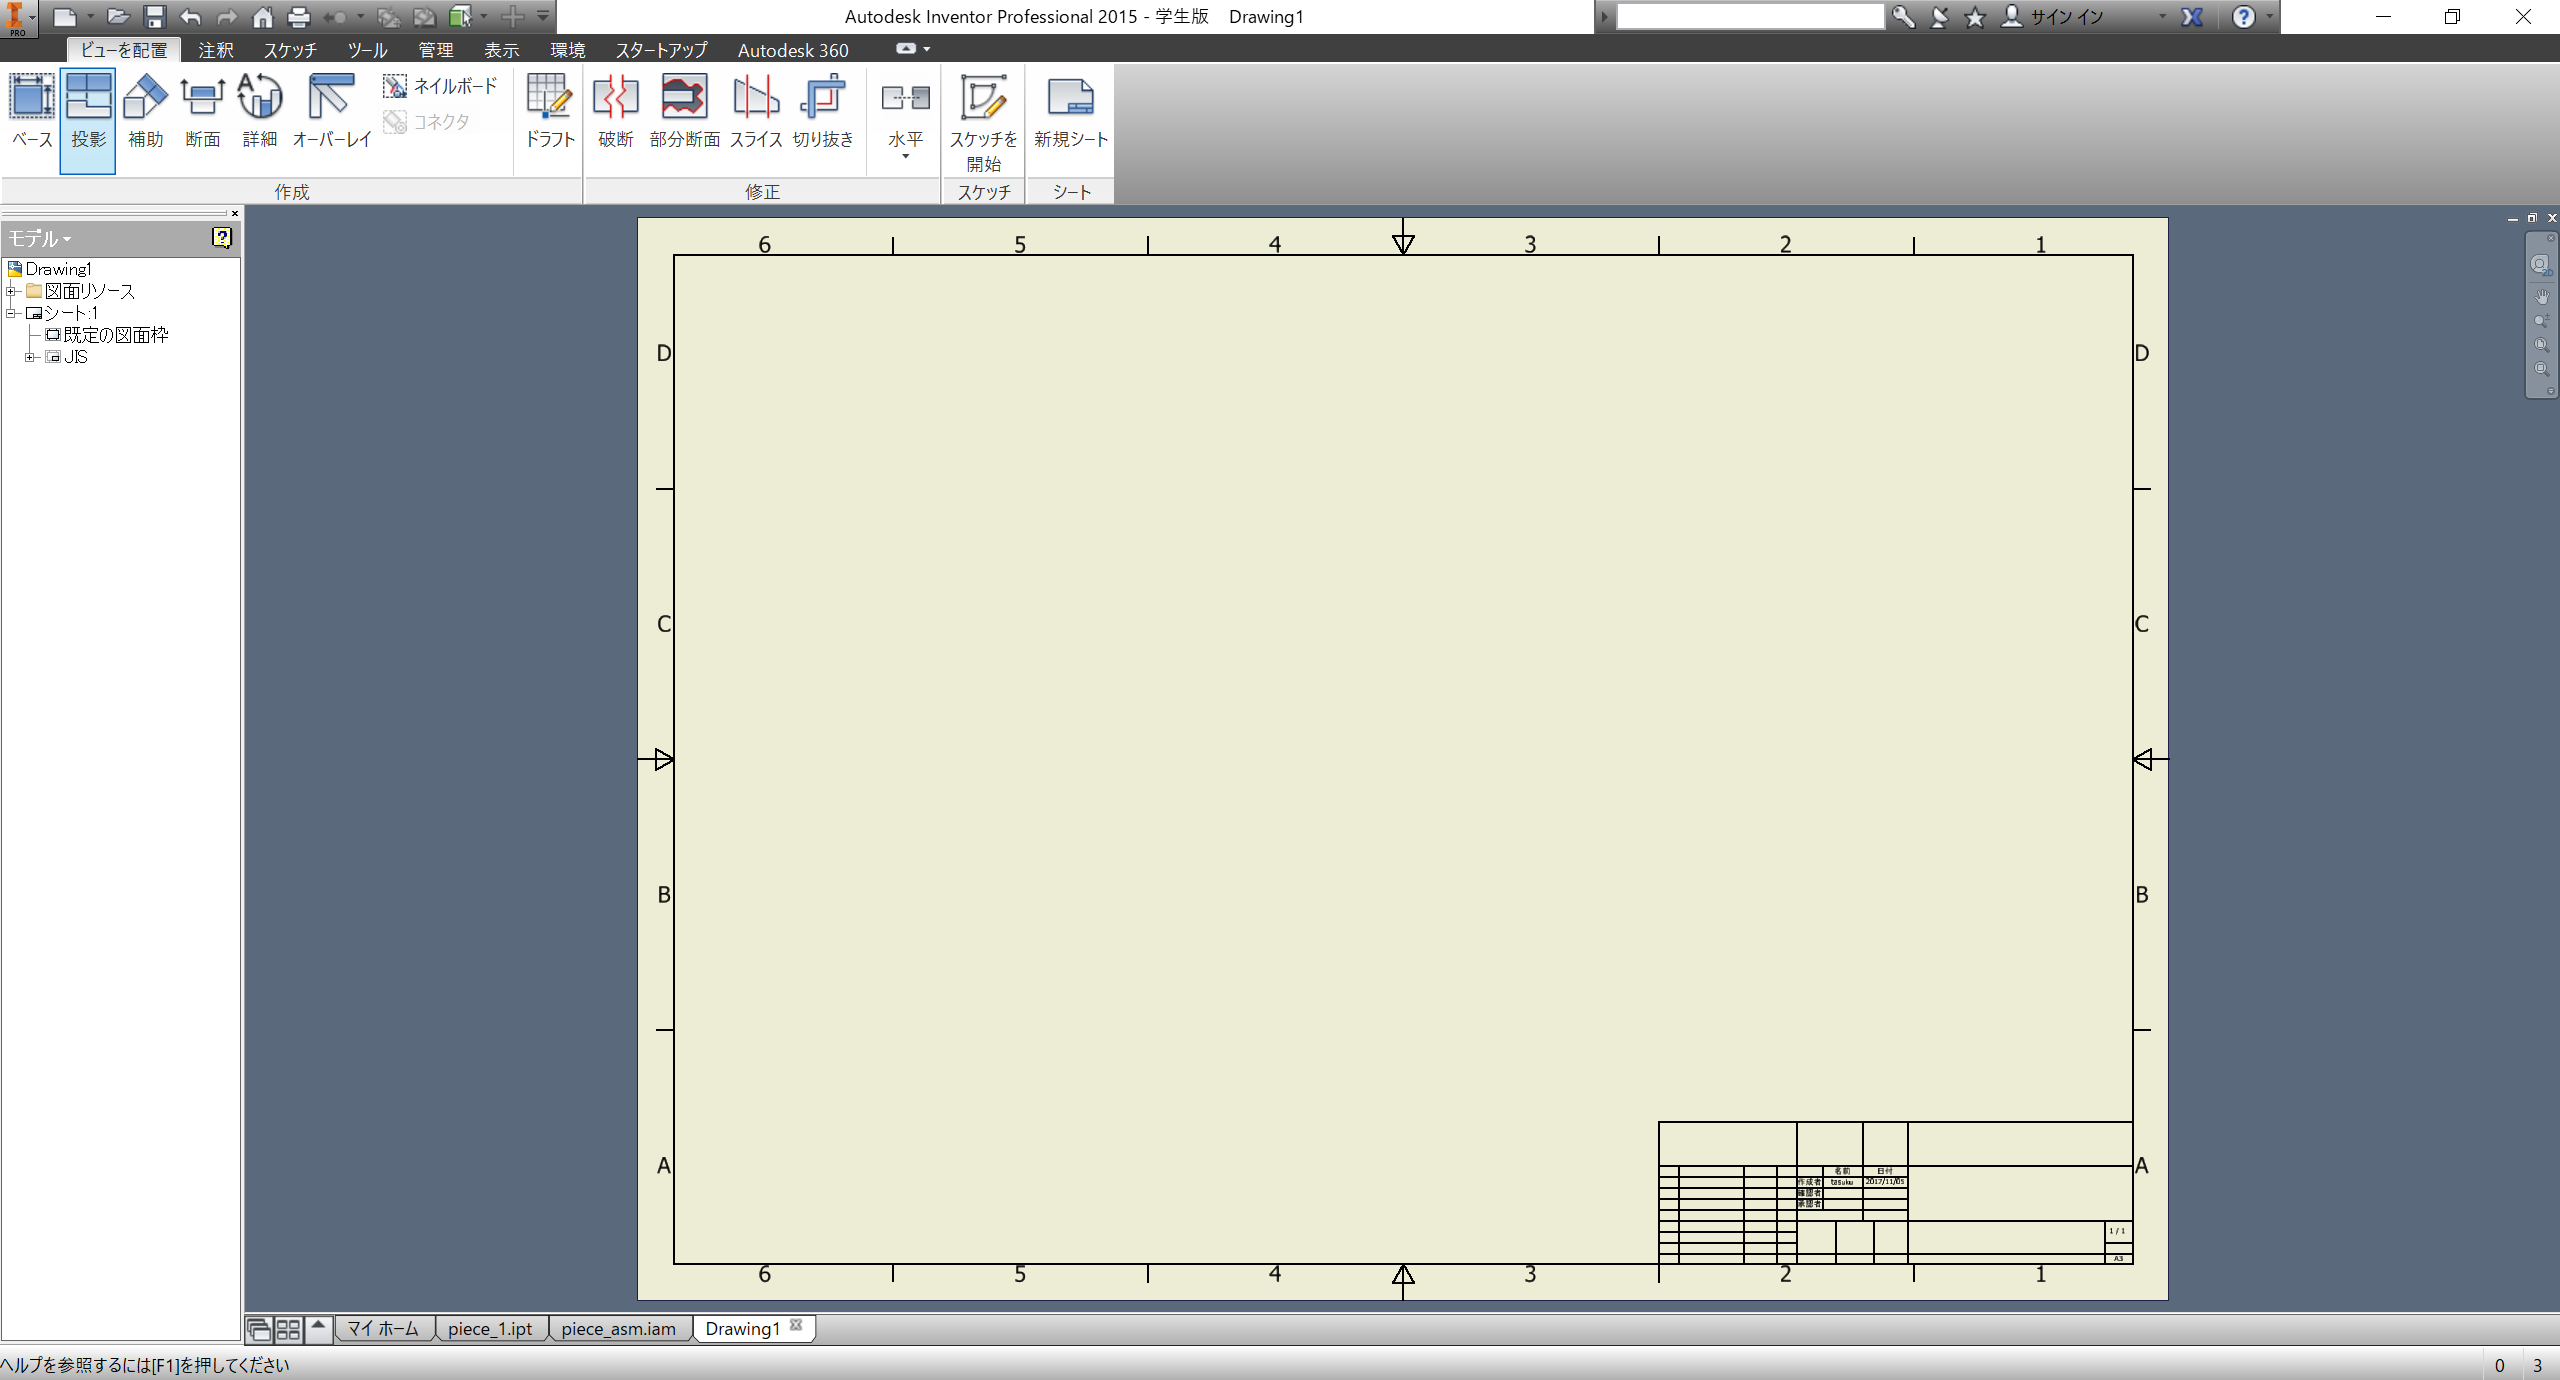
\includegraphics[width=\columnwidth]{plane.png}
   \caption{jpg図の参考例}
  \end{minipage}
  \label{figure:nowprinting}
 \end{center}
\end{figure}

\begin{table}[tbh]
 \begin{center}
  \begin{tabular}{|l|r|} \hline
  A1 & B1 \\
  A2 & B2 \\ \hline
  \end{tabular}
  \caption{図の参考例}
  \label{table:sample}
 \end{center}
\end{table}

\section{各種タイトルでどうしても改行が必要 となる場合の対処法について}

\verb|\section, \subsection|などで改行をしたい場合は単語の間にスペースを入れる.

\section{おわりに}

\bibliographystyle{junsrt}
\bibliography{p-report}


\bibliographystyle{junsrt}
\bibliography{p-report}
\end{document}
